\documentclass[a4paper,12pt]{article}
\usepackage[utf8]{inputenc}
\usepackage[T1]{fontenc}
\usepackage{booktabs}
\usepackage{natbib}
\usepackage{amsmath}
\usepackage{amssymb}
\usepackage[colorlinks=true]{hyperref}
\usepackage[left=2cm]{geometry}
\usepackage{graphicx}

\title{Testing the unguarded X hypothesis}
\begin{document}
\maketitle
\section{Introduction}
The unguarded X (UX) hypothesis states that one reason for females to live longer than males is that they are usually the homogametic sex. This implies that either somatic or inherited (partially) recessive deleterious mutations in the X chromosome are always exposed in males, but concealed in heterozygous females. This hypothesis requires recessive mutations, maintained by mutation-selection balance, that negatively affect longevity both in males and in females. This scenario is hardly controversial. The main uncertainty is whether this kind of mutations can fully explain the difference in longevity between sexes.

The alternative hypothesis is that a different kind of mutations is required to account for the difference in longevity between males and females. Namely, sexually antagonistic mutations, which are maintained at intermediate frequencies in the population by a selection balance. Sexually antagonistic mutations could happen in any chromosome. However, there are theoretical reasons and evidence to belive that they are especially frequent in the X chromosome \citep{Gibson2002}.

\citet{Kelly1999} suggested an experiment to determine if low-frequency, deleterious mutations can explain the observed genetic variance in a character that is correlated with fitness. The alternative is that high-frequency mutations maintained by a selection balance are required to explain the observed variance. It is a qualitative test, rather than a quantitative measure of the contribution of each frequency class. The experiment is relatively easy and it involves a short selection experiment and two short inbreeding experiments. Needless to say that the conclusion would only apply to the population used in the experiment. The test was originaly thought for traits affected mostly by autosomic variation. In section~\ref{sec:autosomic} I explain the theoretical bases of Kelly's test. And in section~\ref{sec:sexlinked} I extend its application to traits mostly affected by X-linked variation.

\section{John K. Kelly's test of the frequency class of deleterious variants}\label{sec:autosomic}
The method is based on a simple model. In every locus (assumed to be autosomic) affecting a trait correlated with fitness, there are a high allele (A$_{1i}$), and a low allele (A$_{0i}$). The three genotypes in one locus, from low to high, have genotypic values $-a_i$, $d_i$, and $a_i$, where $-a_i \leqslant d_i \leqslant a_i$. The frequency of A$_{1i}$ is $p_i$, and that of A$_{0i}$, $q_i$. For simplicity, I drop the $i$ subscript. Under this parameterization, the additive genetic variance contributed by one locus in a population in Hardy-Weinberg equilibrium is $V_a=2pq[a+d(q-p)]^2$ \citet[p. 126]{Falconer1989}.

The other magnitude of interest is the covariance of additive effects with the homozygous dominance effects, $C_{ad}$. The additive effects are what \citet[p. 112]{Falconer1989} calls average effects, say $a_j$ and $a_k$ of alleles $j$ and $k$. The breeding value of an autosomal genotype can be expressed as the sum of the average effects of the two alleles \citep[p.115]{Falconer1989}. And the difference between the breeding value and the genotypic value is the dominance deviation, say $d^j_k$ for genotype $jk$. The homozygous dominance effect of allele $j$ is $d^j_j$, the difference between genotypic and breeding values of genotype $jj$, due to dominance. Thus, the covariance between average effects and homozygous dominance effects, $C_{ad}$ is highest when low alleles (A$_0$) are recessive and high alleles (A$_1$), dominant. \citet{Cockerham1984} defines this covariance for one locus, $i$, as $d_{1i}=\sum_j p_{ji}a_{ji}d^j_{ji}$. This stems from the definition of covariance ($\mathrm{Cov}[a, d]=\mathrm{E}[ad] - \mathrm{E}[a]\mathrm{E}[d]$), and from the fact that the expected average effect among the alleles in one locus ($\mathrm{E}[a]$) is zero. If there are two alleles in the locus, $p_{ji}$ in that formula are $p$ and $q = 1-p$. If $q$ is the frequency of the low allele, A$_0$, then $a_{0i} = -p(a+d(q-p))$, and $a_{1i} = q(a+d(q-p))$. The homozygous dominant effects in this model are $d^0_{0i} = -2p^2d$, and $d^1_{1i}=-2q^2d$ \citep[p. 118]{Falconer1989}. Substituting these values in the formula above, we obtain the expression for $C_{ad}$ given by \citet{Kelly1999}: $C_{ad}=2pq(p-q)d[a+d(q-p)]$.

When several loci are involved, the additive variance is the sum of $V_a$ across loci \citep[p. 129]{Falconer1989}, and the covariance between average effects and homozygous dominance effects, $C_{ad}$, is also the sum of the covariances across all loci \citep{Cockerham1984}. In principle, there are ways to estimate $C_{ad}$ and $V_a$. These quantities are interesting because their ratio, $C_{ad}/V_a$, is sensitive to the allele frequencies. When the low alleles have intermediate frequencies, $C_{ad}/V_a$ drops to values close to or lower than zero. \citet{Kelly1999} proposes a new and efficient way to estimate directly the ratio $C_{ad}/V_a$. Figure~\ref{fig:ratio} shows that a threshold can be chosen on $C_{ad}/V_a$ below which loci with intermediate allele frequencies are likely to contribute to the phenotype.

\begin{figure}
\centering{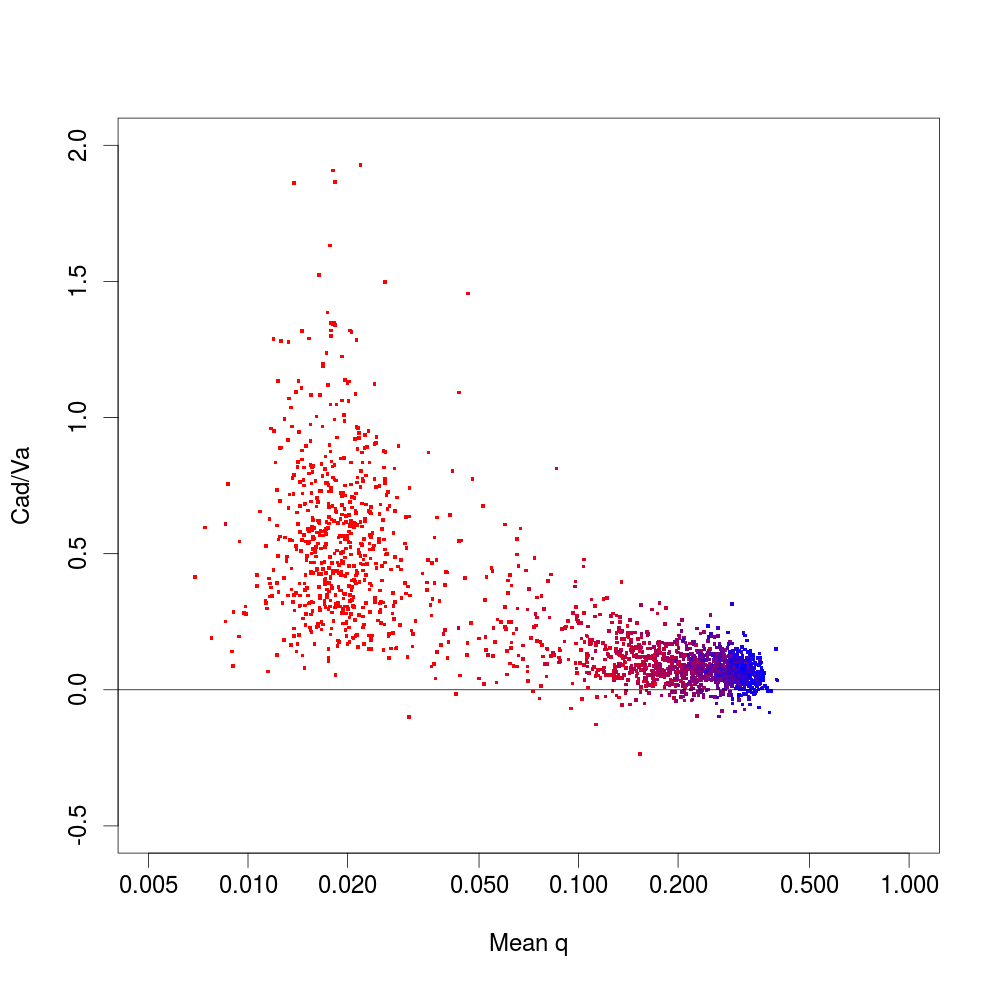
\includegraphics[width=10cm]{../results/2018-01-29/Kelly1999.png}}
\caption{Two thousand simulated $C_{ad}/V_a$ ratios under variable number of loci contributing to the phenotype (between 50 and 200), and a variable proportion of them with intermediate allele frequencies. The colour indicates, from red to blue, the proportion of loci (up to 70\%) the low allele's frequency of which was taken from a Beta distribution with a 0.4 mean}\label{fig:ratio}
\end{figure}

In Kelly's terms, $M$ is the mean phenotype in the population. The directional dominance, $B$, is the difference in mean phenotype between an outbred population and a completely inbred population with the same allele frequencies. $V_a$ is the additive genetic variance, and $V_p$, the total phenotypic variance. $C_{ad}$ is the covariance between the additive effects and the homozygous dominant effects. "The `homozygous dominant effect' is the dominance deviation associated with a particular allele when that allele is in homozygous form." Note that \citet{Cockerham1984} uses the symbol $d_{1i}$ for what Kelly calls $C_{ad}$.

Citing \citet{Kelly1999}, who refers to a character (mostly) affected by autosomal loci: "In the short term, the expected change in the mean phenotype ($M$) equals the product of the cumulative selection differential and the narrow sense heritability \citep{Falconer1989}. The latter is $V_a$ divided by $V_p$, the phenotypic variance. The expected change in the directional dominance ($B$) is the product of the cumulative selection differential and $C_{ad} / V_p$ [...]. Thus, the ratio of the cumulative change in $B$ to the cumulative change in $M$ provides an estimate of the ratio of $C_{ad}$ to $V_a$." And the estimate of $C_{ad}/V_a$ is known to be sensitive to the frequency of partially recessive alleles.

\section{Sex-linked genes}
Dosage compensation in \emph{D. melanogaster} works by doubling the expression of X-linked genes in males, not by inactivating an X chromosome in females. Thus, the genotypic value of a male carrying the A$_1$ allele in its X chromosome can be reasonably assumed to be equal to the genotypic value of the homozygous A$_1$A$_1$ female. Although \citet{James1973} did not know this, he deduced that if that was the case, then the additive genetic variance in males due to a single X-linked locus would be exactly twice the additive genetic variance in females. Actually, his deduction is only correct under his assumption of no dominance. It depends on the heterozygous female having an intermediate genotypic value (see section~\ref{A1}).

The \emph{Drosophila} dosage compensation system also suggests that the concept of dominance among heterozygous females is the familiar one, because all cells in a female express the same genotype. Thus, the additive variance contributed by an X-linked gene among females is the same as that of an autosomal gene in the whole population. And the covariance between allelic effects and homozygous dominant effects is also equivalent (section~\ref{A1}). Thus, the ratio between them, $\sigma(\alpha_F, \delta)/\sigma^2(A'_F)$ must also be sensitive to the average minor allele frequency.

The question is if we can estimate that ratio by the ratio between the cumulative change in directional dominance and the response in the mean phenotype. The directional dominance, $B$, is the difference in mean phenotype between an outbred and a completely inbred population with the same allele frequencies. It is also defined by \citet{Kelly1999b} as the expected value of the homozygous dominance deviation, $b$, among individuals. The individual homozygous dominance deviation, $b$, is the sum of locus-specific homozygous dominance deviations. This, in turn, is the average of the dominance effects that the two alleles present in a locus would have in homozygosity. If the locus is homozygous, the locus-specific homozygous dominance deviation is equal to the dominance effect. In symbols: $B = E(b) = \sum_l \sum_{jk} p_{jl}p_{kl}(\delta _{jjl}+\delta _{kkl})/2$. If all loci are biallelic, $p_k = 1-p_j$, and the previous expression reduces to $B=\sum_l (p_{jl}\delta _{jjl} + q_{kl}\delta _{kkl})$. %I deduce that for a single locus it must be equal to the heterozygous dominance deviation, $\delta_{12}=-pq(a-2d)$. However, \citet{Kelly1999} uses the definition with alternative sign, which in my terms is equivalent to $\mu_I - \mu = pq(a-2d)$. That is, inbreeding reduces the average phenotype. This stems from the assumption that the high allele is at least partially dominant ($a/2 \leq d$). 
The definition and expected value of $B$ due to X-linked genes among females is completely equivalent to that due to autosomal loci in the whole population. However, the expected change of $B$ after selection is deduced in \citet{Kelly1999b} assuming linkage equilibrium. Given that here we are concerned in the contribution of X-linked genes, it would not be appropriate to assume linkage equilibrium, even if we allow for recombination. I need to determine how $B$ and the average phenotype are expected to change after selection with sex-specific transmission and linkage.


%I want to note that \citet{Charlesworth1996} assume frequencies of mutant alleles are low, even though they may affect survival only late in life. This is also an assumption we need to justify the application of Kelly's method to test the UX hypothesis. It could be questioned, because a low selection coefficient against such mutations suggests they could behave as (almost) neutral and eventually drift to not-so-low frequencies.

%\citet{Mukai1974} considers a locus affecting fitness, and therefore uses a different parameterization. The genotypic values (fitness) corresponding to genotypes A$_2$A$_2$, A$_1$A$_2$, and A$_1$A$_1$ (again in increasing order) are now $1-s$, $1-hs$, and 1, respectively. In this case, assuming Hardy-Weinberg equilibrium, the average genotypic value is $1-2pqhs-q^2s$. Note that in this case we could also assume that the population is at mutation-selection equilibrium. Then, according to classic theory, the frequency of A$_2$ should be something like $\mu/hs$.

\section{The experiment}
A sex-linked trait has different genetic variances in males and females. If the trait is defined as sex-specific, and therefore selected only in one sex, the expected change in mean (sex-specific) phenotype would still be the product of the cumulative selection differential and the narrow sense (sex-specific) heritability (I think, because this expectation stems only from the definition of heritability \citep[page XX]{Falconer1989}). This may be the only way to target female longevity, irrespectively of its correlation with male longevity. However, in a population of flies, it is unfeasible to manually select individuals according to the longevity of their mother. Even if individual flies could be marked with their mother's code, marking and reading the codes would not be easier than having the population separated in sex- and family-specific bottles, which is undesirable. A more efficient solution is required. Actually, the literature suggests some options.

\citet[p. 19]{Lund-Hansen2017} claims to be the first case of sex-limited evolution in \emph{Drosophila} that targets females, instead of males. Furthermore, she limits evolution to the X chromosome. That's exactly what we need. Her purpose is just to eliminate male selection on the X chromosome. The female-limited X-chromosome evolution experiment releases sexually antagonistic standing genetic variation from the selection balance, and allows the fixation of alleles beneficial to females in the X chromosome. She accomplishes this by using an X-chromosome balancer and a smart design of crosses. For details, see chapter 2 of \citet{Lund-Hansen2017}, which is available online \href{http://sro.sussex.ac.uk/70184/1/Lund-Hansen%2C%20Katrine%20Koch.pdf}{here}.
First, she introgresses an X-chromosome balancer (FM) into the source population (12 generations of back-crossing). The introgressed population provides a source of males with an FM X-chromosome (FM/Y). In her experiment, a population is a set of 14 vials, with 16 males and 16 females each. In the experimental evolution group, females in a vial are heterzygous FM/X, and the males are FM/Y, so that all the daughters inherit an evolving X chromosome from their mother and an FM balancer from their father. Females must be collected as virgins every generation. In order to allow recombination among evolving X chromosomes, every generation a subset of 16 FM/X females where mated not with FM/Y males, but with X/Y males from the same population. The two evolving X chromosomes in any of their daughters would recombine. When mated with FM/Y males, they would produce FM/X daughters that would go back to the selective regime, one to each of the 14 vials. On the side, Lund-Hansen raised two types of control populations. Each of the three types of populations was replicated four times. That makes $3\times 4 \times 14 = 168$ vials. The experiment went on over 40 generations.

For our purpose, in the populations undergoing female-limited X-chromosome evolution we would have to select for longevity. I think that 20 generations should be enough. 

To summarize, we would need to: 1) run an inbreeding experiment from the source population to estimate $B$ before the selection experiment; 2) measure the average female longevity in the source population; 3) run a female-limited X-chromosome evolution experiment selecting for female longevity; 4) measure the average female longevity after the selection experiment; and 5) run a second inbreeding experiment from the evolved population. Actually, the `inbreeding experiments' would be as short as two or three generations, because they need to affect only the X chromosome. An FM/X female, carrying the X chromosme targeted from homozygosity, would be crossed with an unrelated FM/Y male. Among the progeny, an X/Y male would be crossed with an FM/X sister. The X/X progeny would be homozygous for the whole X chromosome. However, the parents being siblings, the other chromosomes would also be partially inbred. To minimize the contribution from autosomes, half-siblings could be used.


\section{Apendix}
\subsection{X-linked single locus}\label{A1}
The model of genotype values at one X-linked locus specified on table~\ref{tau:values} differs from that of \citet{James1973} only in that here the heterozygous females have $G_{F12}'=d$, while in \citet{James1973}, $G_{F12}' = a/2$. My model just allows for dominance, while James assumed an intermediate phenotype in the heterozygous females.

\begin{table}
\begin{center}
\caption{Model of genetic values. The genic effects ($\alpha$ terms below) are defined as the average deviation from the sex-specific population's mean produced by each allele. They are: $\alpha_{M1}'=qb$, $\alpha_{M2}'=-pb$, $\alpha_{F1}'=pqa - qd(p-q)$, and $\alpha_{F2}'=-p^2a + pd(p-q)$. It can be noticed that dominance deviations (in females) vanish in the absence of dominance ($d=a/2$). The prime symbol is used to denote X-linked genes, as in \cite[chapter 24]{Lynch1998}}\label{tau:values}
\begin{tabular}{lccccc}
\toprule
&\multicolumn{3}{c}{Females}&\multicolumn{2}{c}{males}\\
\midrule
Genotypes&A$_1$A$_1$&A$_1$A$_2$&A$_2$A$_2$&A$_1$&A$_2$\\
Frequencies&$p^2$&$2pq$&$q^2$&$p$&$q$\\
Genotypic values&$a$&$d$&0&b&0\\
\cmidrule(lr){2-4}\cmidrule(lr){5-6}
Average values&\multicolumn{3}{c}{$\mu_F=p^2 + 2pqd$}&\multicolumn{2}{c}{$\mu_M=pb$}\\
\cmidrule(lr){2-4}\cmidrule(lr){5-6}
Estimated values&$\mu_F + 2\alpha_{F1}'$&$\mu_F + \alpha_{F1}' + \alpha_{F2}'$&$\mu_F + 2\alpha_{F2}'$&$\mu_M + \alpha_{M1}'$&$\mu_M + \alpha_{M2}'$\\
Dominance deviations&$q^2(2d - a)$&$-pq(2d-a)$&$p^2(2d-a)$&0&0\\
\bottomrule
\end{tabular}
\end{center}
\end{table}

In males, all genetic variance is addititve. Because the sex-specific average genic effect is 0, the variance of genic effects is just the expected square of genic effects. Thus, in males, $\sigma^2(A_M')=\sigma^2(\alpha_{Mi}')=\sum p_i(\alpha_{Mi}')^2=pqb^2$. In females, where $G_{Fij}'=\mu_F + \alpha_{Fi}' + \alpha_{Fj}' + \delta_{ij}'$ the genetic variance has an additive and a dominance component, $\sigma^2(G_F')=\sigma^2(A_F') + \sigma^2(D_F')$, where $\sigma^2(A_F')=2pq(p^2(a-d)^2 + 2pq(a-d)d + q^2d^2)$. This assumes uncorrelated genic effects, which should be the case under random mating. If $d = a/2$, the females additive variance reduces to $\frac{1}{2}pqa^2$, which would be exactly half the male genetic variance if $a = b$ and $d=\frac{a}{2}$. 

The relationship between male and female X-linked additive variances has been a recurrent topic in the literature. \citet{James1973} favoured the hypothesis that $a=b$ due to dosage compensation, in which case $\sigma^2(A_M') = 2\sigma^2(A_F')$. And he claims that "the reason is that in females the genetic values are averages of two genic values, the variance of the averages being half the variance of individual values." This seems to contradict a statement from the previous page in the same article: "a female genetic value is the sum of two genic values". However, the same argument is reproduced by \citet{Reinhold2013}, who base their whole article on the idea that the heterogametic sex should be more variable. Even \citet[pp. 715f]{Lynch1998} are quite ambiguous about this. The fact is that the relationship between $\sigma^2(A_F')$ and $\sigma^2(A_M')$ depends on dominance and gene frequencies. With strong dominance ($d\sim a$ or $d\sim 0$) the female variance can be higher than the male one. Figure~\ref{fig:variances} is very similar to figure~1 in \citet{Reinhold2013}. Certainly, the parameter space where female variance is higher is not very large. If the low allele, A$_2$, is completely recessive ($d=a$) and at low population frequency (high $p$), as expected by slightly deleterious alleles, the female variance is expected to be negligible.

\begin{figure}
\centering{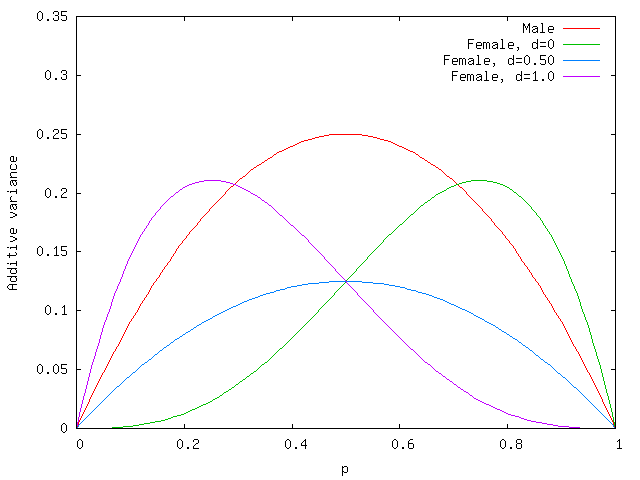
\includegraphics[width=7cm]{variances.png}}
\caption{Additive genetic variances corresponding to one bi-allelic, X-linked locus in males and in females, with or without dominance. With $d=0$, allele A$_2$ is completely dominant. With $d=0.5$, there is no dominance. With $d=1$, allele A$_1$ dominates. The $p$ on the X axis is the frequency of A$_1$.}\label{fig:variances}
\end{figure}

Under the model specified on table~\ref{tau:values}, the covariance between the average effects and the homozygous dominant effect is $\sigma(\alpha_F,\delta) = pq(a-2d)(q-p)(pa-d(p-q))$. This covariance only exists among females. The formula is equivalent to what it would be for autosomal loci among the whole population.



\bibliographystyle{abbrvnat}
\bibliography{ux}

\end{document}
